\chapter{Introduction}\label{CH:introduction}
Above Earth's atmosphere are the Van Allen radiation belts, a toroidally-shaped pair of belts that consist of a complex and dynamic plasma environment. The inner radiation belt is stable, consists of mostly energetic protons, and is located within 2 Earth radii (measured near the equator) above Earth's surface. The outer radiation belt, on the other hand, consists of mostly energetic electrons, is highly dynamic on day and hour time scales, and is typically found between 4 and 8 Earth radii above Earth's surface. These belts pose a threat to space exploration due to their adverse effects on our bodies and electrical components. A few \textcolor{red}{effects} include: a high radiation dose for manned missions, degradation of silicon that causes transistor malfunction, computer memory corruption due to bit flips, etc. With these effects in mind, it is no surprise that the radiation belts have been extensively studied since their discovery in the 1960s.

The radiation belt particles, mostly consisting of electrons and protons, are at times unstable to wave growth and generate electric and magnetic waves. These waves can then accelerate and scatter radiation belt particles with a variety of wave-particle mechanisms. These wave-particle interactions are believed to be responsible for scattering electron microbursts, a short and intense increase of precipitating electrons into Earth's atmosphere, that are capable of destroying ozone molecules and rapidly deplete the outer belt's electrons.

Electron microbursts, henceforth referred to as microbursts, are typically observed by low Earth orbiting spacecraft, sounding rockets, and high altitude balloons as a sub-second impulse of electrons. Some of the most intense microbursts have electron fluxes that are a factor of 10 to 100 above the background (for example see Fig. 7 in \citet{Blake1996}). Since they were first reported by \citet{Anderson1964}, the intense transient nature of microbursts have compelled countless researchers to pursue an understanding of their properties, their effects on the environment, and the physical mechanism(s) that create microbursts. Microbursts are widely believed to be created by wave-particle scattering between a plasma wave called whistler mode chorus and outer radiation belt electrons, although many details regarding the scattering mechanism are unconstrained or unknown. The goal of this dissertation is to expand our knowledge of the wave-particle scattering mechanism that scatters electron microbursts.

This chapter serves as an introduction to the fundamental physical concepts that are essential to understand wave-particle interactions in Earth's magnetosphere. We will review the motion of charged particles in electric and magnetic fields, how particles are organized in the magnetosphere, how particles are accelerated and lost in the magnetosphere, and review the current state of our understanding of microbursts.

Then the rest of this dissertation expands our knowledge of microbursts. In Chapter \ref{CH:mageis_microburst} \textcolor{red}{(chapter numbers will be filled in the full dissertation)} we will investigate and model the scattering mechanism responsible for microbursts observed inside the outer radiation belt, near the magnetic equator. Then in Chapters \ref{CH:bouncing_packet} and \ref{CH:ac6_study} we will investigate the microburst scattering mechanism indirectly by estimating the microburst footprint size in low Earth orbit and the magnetic equator (near where microburst electrons are believed to be scattered) and compare it to sizes of chorus waves estimated in prior literature.

\section{Charged Particle Motion in Electric and Magnetic Fields}\label{Intro:particle_motion}
A charged particle trapped in the magnetosphere will experience three types of periodic motion in Earth's nearly dipolar magnetic field in the absence of electric fields. The three motions are ultimately due to the Lorentz force that a particle of momentum $\vec{p}$, charge $q$, and velocity $\vec{v}$ experiences in an electric field $\vec{E}$ and magnetic field $\vec{B}$ and is given by
\begin{equation} \label{Intro:Lorentz}
\frac{d\vec{p}}{dt} = q(\vec{E} + \vec{v} \times \vec{B}).
\end{equation} In the magnetosphere, the three periodic motions, in decreasing frequency, are gyration, bounce, and drift and are schematically shown in Fig. \ref{Intro:motion_diagram}. Each periodic motion has a corresponding conserved quantity i.e. an adiabatic invariant. 

\begin{figure}
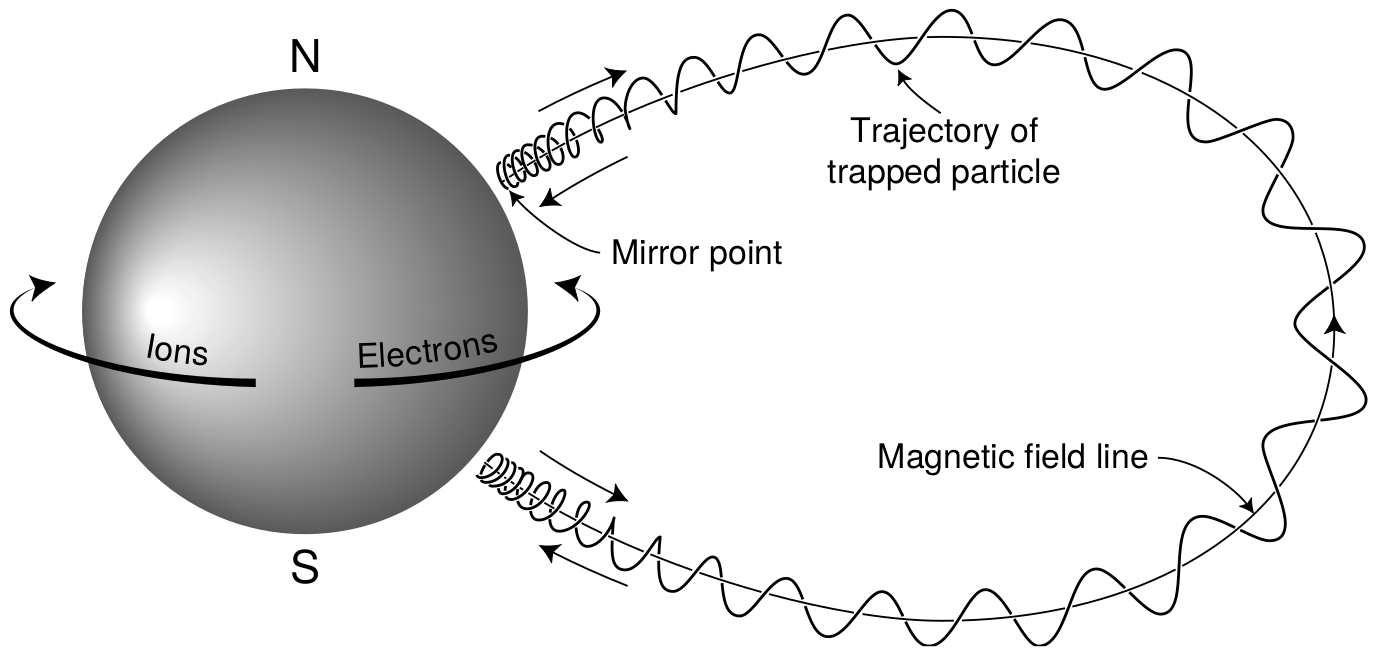
\includegraphics[width=\textwidth]{1_three_motions.png}
\caption{The three periodic motions of charged particles in Earth's dipole magnetic field. These motions are: gyration about the magnetic field line, bounce motion between the magnetic poles, and azimuthal drift around the Earth. Figure from \citep{Baumjohann1997}.}
\label{Intro:motion_diagram}
\end{figure}


The highest frequency periodic motion is gyration about a magnetic field of magnitude $B$. This motion is circular with a Larmor radius of 
\begin{equation}
r = \frac{m v_\perp}{|q| B}
\end{equation} where $m$ is the mass and $v_\perp$ the particle's velocity perpendicular to $\vec{B}$. This motion has a corresponding gyrofrequency of
\begin{equation}
\Omega = \frac{|q| B}{m}
\end{equation} in units of radians/second. In the radiation belts, the electron gyrofrequency, $\Omega_e$, is on the order of a kHz. The corresponding adiabatic invariant is found by integrating the particle's canonical momentum around the particle's path of gyration,
\begin{equation} \label{J}
J_i = \oint (\vec{p} + q \vec{A}) \cdot d\vec{l}
\end{equation} where $J_i$ is the $i^{th}$ adiabatic invariant and $\vec{A}$ is the magnetic vector potential. This integral is carried out by integrating the first term over the circumference of the gyro orbit and integrating the second term using Stokes theorem to calculate the magnetic flux enclosed by the gyro orbit.  The gyration invariant is $J_1 \sim v_\perp^2 / B$ which is conserved when the frequency, $\omega$, of a force acting on the gyrating electron satisfies $\omega << \Omega_e$.

The second highest frequency periodic motion is bouncing due to a parallel gradient in $\vec{B}$. This periodic motion naturally arises in the magnetosphere because Earth's magnetic field is stronger near the poles. To understand this motion we first we need to define the concept of pitch angle, $\alpha$ as the angle between $\vec{B}$ and $\vec{v}$ which is schematically shown in Fig. \ref{Intro:pa}a. The pitch angle relates $v$ with $v_\perp$ and $v_{||}$, the component of the particles velocity parallel to $\vec{B}$. As shown in Fig. \ref{Intro:pa}b and \ref{Intro:pa}c, a smaller (larger) $\alpha$ will increase (decrease) the distance that the charged particle travels parallel to $\vec{B}$ during one gyration.

Assuming the particle's kinetic energy is conserved, the conservation of $J_1$ implies that given a particle's $v_\perp(0)$ and $B(0)$ at the magnetic equator (where Earth's magnetic field is usually at a minimum) we can calculate its $v_\perp(s)$ along the particle's path, $s$, by calculating $B(s)$ from magnetic field models. Thus the particle's perpendicular velocity is then related via
\begin{equation} \label{j1_conservation}
\frac{v_\perp^2 (0)}{B(0)} = \frac{v_\perp^2 (s)}{B(s)}
\end{equation} which can be rewritten as 

\begin{equation}
\frac{v^2 \sin^2{\alpha(0)}}{B(0)} = \frac{v^2 - v^2_{||}(s)}{B(s)}
\end{equation} and re-arranged to solve for $v_{||}(s)$ by

\begin{equation} \label{Intro:eq_vp} 
v_{||}(s) = v \sqrt{1 - \frac{B(s)}{B(0)} \sin^2{\alpha(0)}}
\end{equation} which will tend towards 0 as the second term in the radical approaches 1.

The location where $v_{||}(s) = 0$ is called the mirror point and is where a particle reverses direction. Since Earth's magnetic field is stronger towards the poles, the mirroring particle will execute periodic bounce motion between its two mirror points in the northern and southern hemispheres. The corresponding adiabatic invariant, $J_2$ is

\begin{equation} \label{Intro:j2}
J_2 = \oint p_{||} ds
\end{equation} where $ds$ describes the particle path between the mirror points in the northern and southern hemispheres (see Fig. \ref{Intro:motion_diagram}). $J_2$ is found by substituting Eq. \ref{Intro:eq_vp} into Eq. \ref{Intro:j2} and defining the magnetic field strength at the mirror points as $B_m$ (where $\alpha(m) = 90^\circ$). The $J_2$ integral can be written as     
\begin{equation}
J_2 = 2 p \int_{m_n}^{m_s} \sqrt{1 - \frac{B(s)}{B(m)}} ds
\end{equation} where $m_n$ and $m_s$ are the northern and southern mirror points, respectively. The bounce period can be estimated \citep[e.g.][]{Baumjohann1997} to be 

\begin{equation}
t_b \approx \frac{L R_e}{\sqrt{W/m}} (3.7 - 1.6 \sin{\alpha(0)})
\end{equation} where $W$ is the particle's kinetic energy, and $L$ is the $L$-shell. The $L$-shell is the distance from the Earth's center to the location where a particular magnetic field line crosses the magnetic equator, in units of Earth radii, $R_e$. As with gyration, the particle will bounce between the mirror points as long as $\omega << \Omega_b$, where $\Omega_b$ is the bounce frequency.

At this stage it is instructional to introduce loss cone pitch angle, $\alpha_L$.  Conventionally, the loss cone pitch angle is defined as the pitch angle where a particle will mirror at $\approx 100$ km altitude in the atmosphere. A charged particle gyrating at those altitudes will encounter and Coulomb scatter with the dense atmosphere and be lost. The $100$ km altitude is only a convention and not a hard boundary, e.g. the peak in the 1 MeV electron ionization rate is at $\approx 60$ km altitudes \citep{Fang2010}.

\begin{figure}
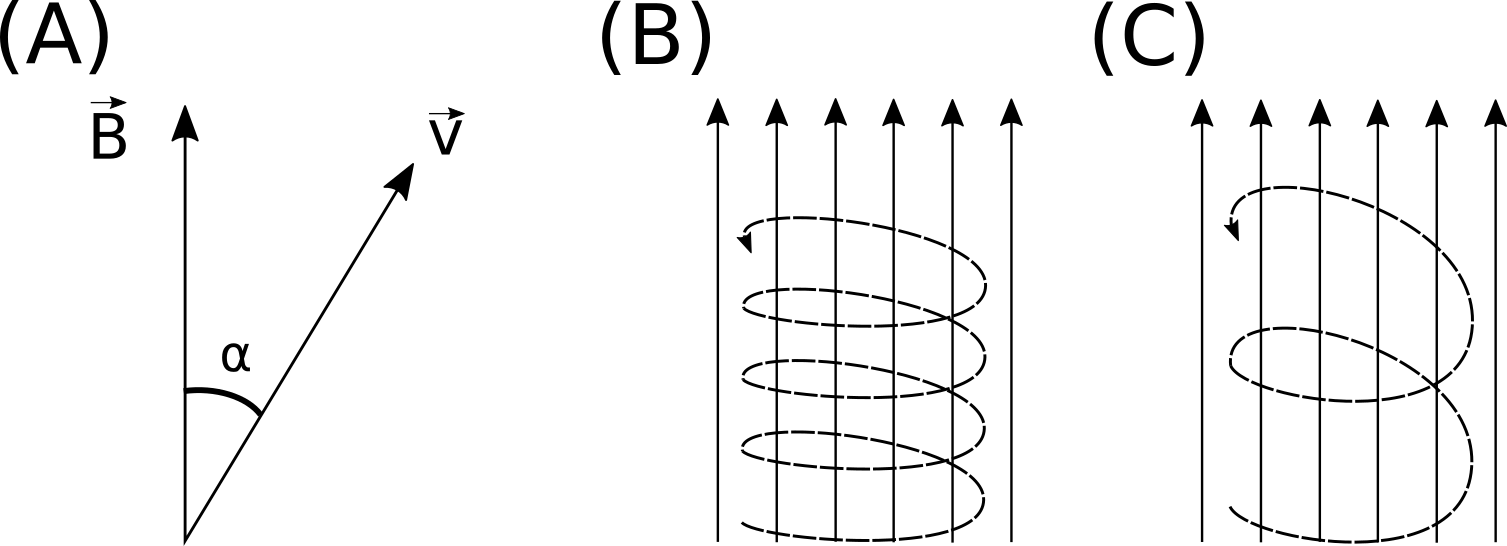
\includegraphics[scale=1]{1_pitch_angle_and_helix.png}
\caption{Charged particle motion in a uniform magnetic field $\vec{B}$. Panel (A) shows the geometry defining the pitch angle, $\alpha$. Panel (B) and (C) show two helical electron trajectories with dashed lines assuming a large and small $\alpha$ (corresponding to a small and large parallel velocity $v_{||}$), respectively.}
\label{Intro:pa}
\end{figure}

The slowest periodic motion experienced by charged particles in Earth's magnetic field is azimuthal drift around the Earth. This drift primarily results from a combination of a radial gradient in $\vec{B}$ and the curvature of the magnetic field. The radial gradient drift arises because Earth's magnetic field is stronger near the Earth. The particle's gyroradius shrinks as it gyrates towards Earth, and expands when it gyrates away from Earth. The overall effect is the particle gyro orbit does not close on itself causing eastward drift of negatively charged particles and westward drift of positively charged particles. The radial gradient drift is further enhanced by the centrifugal force that a particle experiences as it bounces along the curved field lines. The drift adiabatic invariant, $J_3$ is found by integrating Eq. \ref{J} over the complete particle orbit around the Earth. The shape of this drift orbit is known as a drift shell, and can be visualized by rotating the trapped particle trajectory in Fig. \ref{Intro:motion_diagram} around the axis that connects the poles. For $J_3$, the first term is negligible and the second term is the magnetic flux enclosed by the drift shell, $\Phi_m$  i.e. $J_3 \sim \Phi_m$ \textcolor{red}{Add the $J_3$ derivation}. 

To quantify the frequencies of the three periodic motions, Fig. \ref{Intro:adiabatic_frequencies} from \citet{Schulz1974} shows contours of the gyration, bounce, and drift frequencies for electrons and protons in Earth's dipole magnetic field. 

\begin{figure}
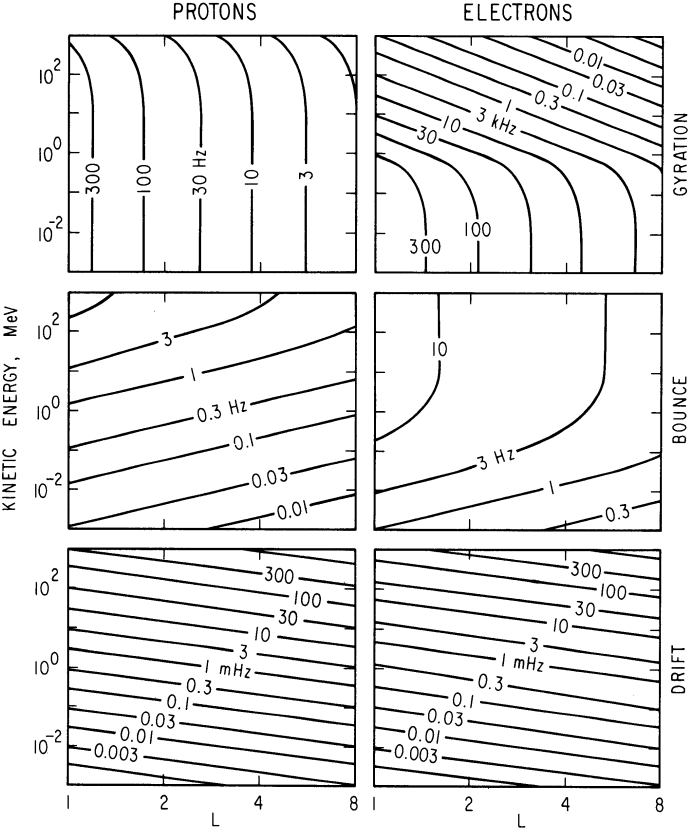
\includegraphics[width=\textwidth]{1_schulz_lanzerotti_fig6.png}
\caption{Contours of constant gyration, bounce, and drift frequencies for electrons and protons in a dipole field. Figure from \citet{Schulz1974}.}
\label{Intro:adiabatic_frequencies}
\end{figure}

Up until now we have considered the three periodic motions due Earth's magnetic field in the absence of electric fields. If there is an electric field, $\vec{E}$, perpendicular to $\vec{B}$, a particle's center of gyration (averaged position of the particle over a gyration) will drift with a velocity perpendicular to both $\vec{E}$ and $\vec{B}$. The drift velocity can be solved using Eq. \ref{Intro:Lorentz} and is
\begin{equation}
\vec{v}_E = \frac{\vec{E} \times \vec{B}}{B^2}.
\end{equation} If there is a parallel magnetic field, $E_{||}$, then the particle is accelerated along the magnetic field line. An $E_{||}$  pointing away from the Earth will contribute to the mirror force and raise the particle's mirror point. On the contrary, an Earthward pointing $E_{||}$ will oppose the mirror force and lower the mirror point. If the Earthward $E_{||}$ lowers the mirror point into the atmosphere, those particles will precipitate into the atmosphere. This is the mechanism that generates the aurora.
        
\section{Particle Populations and Their Interractions in the Magnetosphere}\label{ntro:particle_populations}
Now that we have looked at the dynamics of single-particle motion in electric and magnetic fields, we will briefly tour the various macroscopic populations in the magnetosphere that are illustrated in Fig. \ref{Intro:inner_magnetosphere}.

\begin{figure}
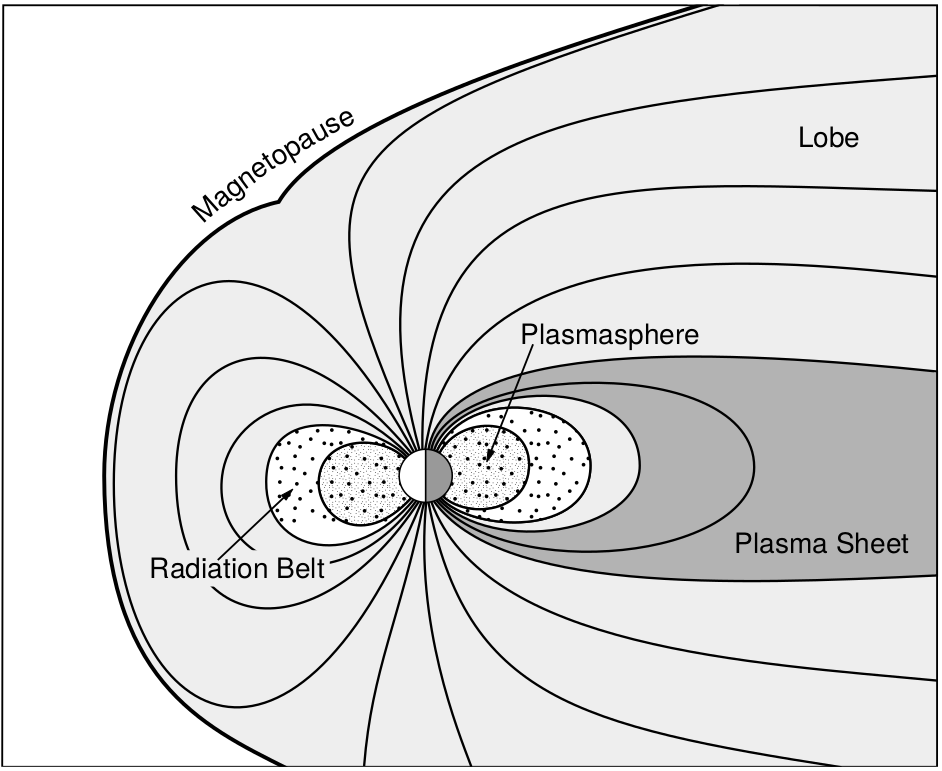
\includegraphics[width=\textwidth]{1_inner_magnetosphere.png}
\caption{A few macroscopic structures in the magnetosphere. The magnetosphere boundary with the solar wind is the magnetopause. The magnetotail consists of two lobes that contain Earth's magnetic flux with the plasma sheet separating the two lobes. The inner magnetosphere contains the plasmasphere, the ring current, and the radiation belts which are co-located. Figure from \citet{Baumjohann1997}.}
\label{Intro:inner_magnetosphere}
\end{figure}

The sun and its solar wind are ultimately the source of energy input into the magnetosphere. The solar wind at Earth's orbit is a plasma traveling at supersonic speeds with an embedded interplanetary magnetic field (IMF). When the solar wind encounters Earth's magnetic field, the plasma can not easily penetrate into the magnetosphere because the plasma is frozen-in on magnetic field lines. The plasma is frozen-in on magnetic field lines because plasma has a nearly infinite conductivity. Thus the plasma and its magnetic field drapes around the magnetosphere, forming a cavity in the solar wind that qualitatively has a shape as shown in Fig. \ref{Intro:inner_magnetosphere}. The solar wind is supersonic at 1 AU so a bow shock exists upstream of the magnetosphere which compresses and heats the solar wind. Downstream of the bow shock, the solar wind plasma flows around the magnetosphere inside the magnetosheath. The magnetopause is the surface where the solar wind ram and Earth's magnetic pressures balance. To first order, the magnetopause can be thought of as a boundary between the solar wind and Earth's magnetosphere. The shocked plasma then flows past the Earth where it shapes the magnetotail. In the magnetotail, the magnetopause exists where the solar wind magnetic pressure balances Earth's magnetic field pressure in the lobes. The magnetotail extends on the order of 100 $R_E$ downstream of Earth, and the tailward stretching of magnetic field lines creates a region where Earth's Earthward and anti-Earthward magnetic fields are in proximity. In this region, the curl of $\vec{B}$ is non-zero, thus by Ampere's law there must be a current (called the plasma sheet) near the magnetic equator \citep[e.g.][]{Eastwood2015}.

\subsection{Populations in the Inner Magnetosphere}\label{Intro:inner_mag}
Closer to Earth, where the magnetic field is largely dipolar, are three plasma populations that comprise the inner magnetosphere: the plasmasphere, the ring current, and the radiation belts which are shown in Fig. \ref{Intro:inner_magnetosphere}. Before we describe these three particle populations in detail, we will introduce the coordinate system that most naturally describes the inner magnetosphere environment, and the electric fields that mostly effect low energy particles.

In this coordinate system the ``radial" coordinate was defined in section \ref{Intro:particle_motion} and is the L shell. The azimuthal coordinate is the magnetic local time (MLT). For an observer above Earth's north pole looking down, MLT is defined to be 0 (midnight) in the anti-sunward direction and increases in the counter-clockwise direction with 6 at dawn, 12 at noon (sunward direction), and 18 in dusk. The final coordinate is the magnetic latitude, $\lambda$, which is analogous to the latitude coordinate in the spherical coordinate system and is defined to be 0 at the magnetic equator. This coordinate system is shown in Fig. \ref{Intro:dipole_coords} and naturally describes the inner magnetosphere populations described below.

\begin{figure}
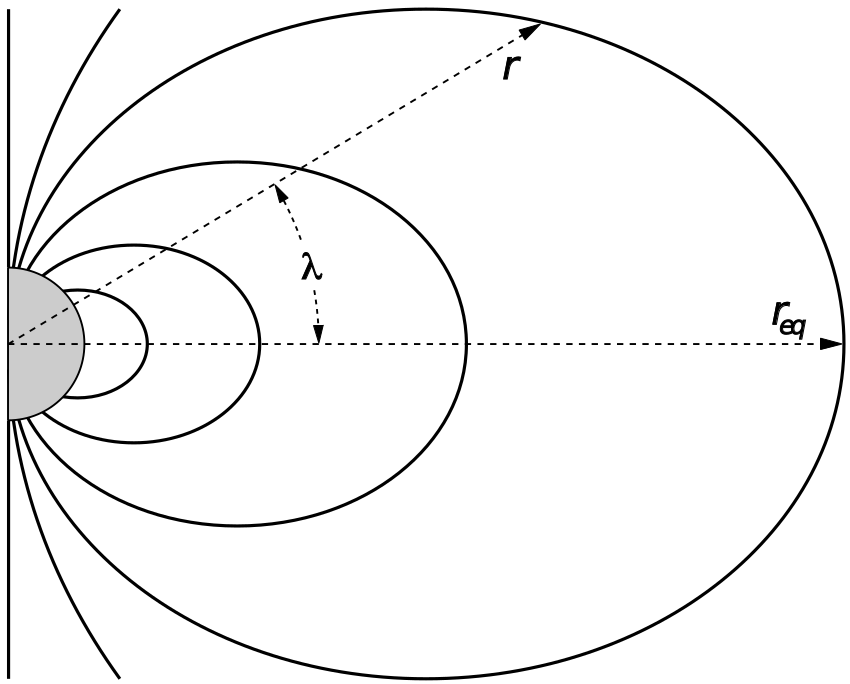
\includegraphics[width=\textwidth]{1_dipole_coords.png}
\caption{The dipole coordinate system. The magnetic latitude of $\mathbf{r}$ is $\lambda$. The radial distance to a magnetic field line in the equatorial plane is typically given by $L = r_{eq}/R_e$. Figure from \citet{Baumjohann1997}.}
\label{Intro:dipole_coords}
\end{figure}


The low energy particle dynamics in the inner magnetosphere are organized by the co-rotation and the dawn-dusk (pointing from approximately $6$ to $18$ MLT) electric fields. The co-rotation electric field arises from Earth's rotation. Earth's magnetic field and the particles frozen on it rotate with the Earth so in the magnetosphere (non-rotating) reference frame the particles appear to $\vec{E} \times \vec{B}$ drift with Earth's rotation. \textcolor{red}{Make sure the E cross B drift is references correctly}. Thus the co-rotation $\vec{E}$ points towards Earth. The other electric field points from dawn to dusk is called the convection electric field and is due to the Earthward transport of particles from the magnetotail. In the magnetosphere reference frame this motion appears as an electric field pointing from dawn to dusk. The superposition of the co-rotation and and convection electric fields is a potential field shown in Fig. \ref{Intro:E_fields}. The shaded area in Fig. \ref{Intro:E_fields} shows where low energy electrons execute closed orbits around Earth (i.e. particles are trapped), and outside this region the particles are not trapped. The dynamic topology of the shaded region in Fig. \ref{Intro:E_fields} is controlled by only the convection electric field which is dependent on the solar wind speed and the IMF. Due to $\vec{E} \times \vec{B}$ drift, the lowest energy particles orbit along equipotential lines in the shaded region in Fig. \ref{Intro:E_fields} and make up the plasmasphere.

\begin{figure}
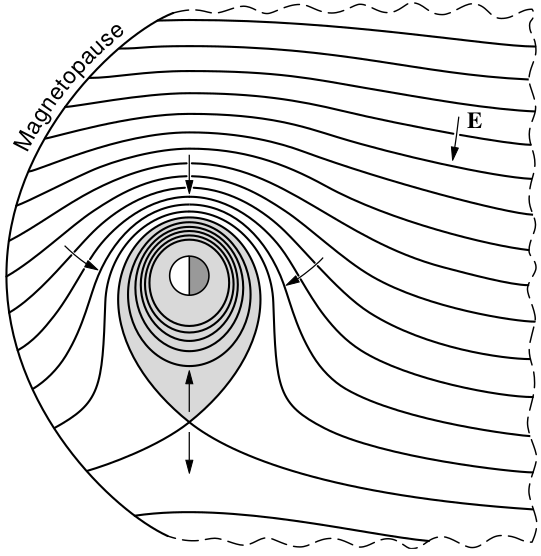
\includegraphics[width=\textwidth]{1_convection_corotation.png}
\caption{Equipotential lines and electric field arrows due to the superposition of the co-rotation and convection electric fields. Electrons in the shaded region execute closed orbits. Outside of the shaded regions the electrons are not trapped and will escape. The region separating the two regimes is called the Alfven layer. Figure from \citet{Baumjohann1997}.}
\label{Intro:E_fields}
\end{figure}

\subsubsection{Plasmasphere}
The plasmasphere is a relatively dense ($n_e \sim 10^3/\mathrm{cm}^3$) and cool ($\sim \mathrm{eV}$) plasma. The plasmasphere typically extends to $L \sim 4$ and the spatial extent is highly dependent on the solar wind and magnetospheric conditions. The source of the plasmasphere is the ionosphere, a layer in Earth's upper atmosphere that contains a high concentration of electrons and ions. The main mechanisms that ionize the ionosphere are ultraviolet light from the sun and particle precipitation. The ultraviolet ionization by sunlight is strongly dependent on the time of day and latitude, while particle precipitation is highly dependent on magnetospheric conditions and mostly occurs at high latitudes.

The outer boundary of the plasmasphere is called the plasmapause which is typically identified by a steep radial gradient in plasma density from $\sim 10^3 / \mathrm{cm}^3$ to $\sim 1 / \mathrm{cm}^3$. It is important to know the location of the plasmapause since the plasma density strongly controls the efficiency of particle scattering by waves. For example, electron scattering by chorus waves is more efficient when the ratio of the plasma and gyro frequency is low which is typically found in low plasma density regions outside of the plasmapause \citep[e.g.][]{Horne2003c, Horne2005, O'Brien2003empirical}.

\subsubsection{Ring Current}
A higher energy population is the ring current. This population consists of protons and electrons between tens and a few hundred keV that drift around the Earth. The orbits of higher energy particles are not as affected by the convection and co-rotation electric field, instead they drift around the Earth due to gradient and curvature drifts. Since the direction of the drift is dependent on charge, protons drift west around the Earth and electrons drift East. This effect creates a current around the Earth. 

The ring current generates a magnetic field which decreases the magnetic field strength at the surface of the Earth and increases it outside of the ring current. The decrease of Earth's magnetic field strength is readily observed by a system of ground-based magnetometers and is merged into a Disturbance Storm Time (DST) index to quantify the global reduction in the magnetic field. An example of a DST index time series from the 2015 St. Patrick's Day storm, driven by a coronal mass ejection (CME), is shown in Fig. \ref{Intro:dst}. A few notable features of the storm and the ring current are worth mentioning. At the start of the storm the ring current is sometimes depleted and DST increases slightly (termed the initial phase or sudden storm commencement) and is shown by the red horizontal bar in Fig. \ref{Intro:dst}. During the main phase of the storm the ring current population is rapidly built up and DST rapidly decreases which is shown by the green bar in Fig. \ref{Intro:dst}. After the storm passes, the ring current gradually decays toward its equilibrium state over a period of a few days and DST returns towards zero during the recovery phase which is shown by the blue bar in Fig. \ref{Intro:dst}. The DST index, along with other geomagnetic indicies, are used by the space physics community to quantify the global state of the magnetosphere.

\begin{figure}
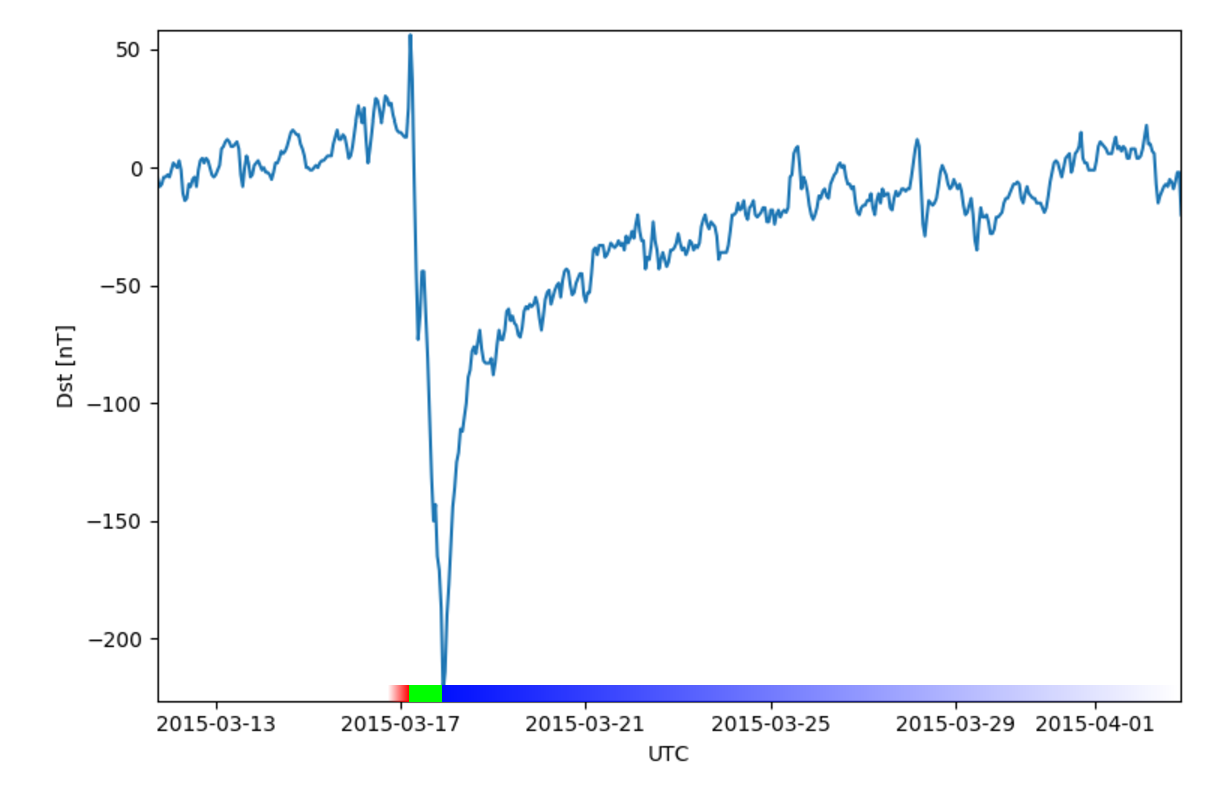
\includegraphics[width=\textwidth]{1_dst.pdf}
\caption{The DST index during the St. Patrick's Day 2015 storm. This storm was caused by a coronal mass ejection on March 15th, 2015. The storm phases are: initial phase, main phase, and recovery phase. The initial phase occurred when the Dst peaked at +50 nT on March 17th during which the ring current was eroded by the coronal mass ejection during the interval shown by the red bar shown at the bottom. Then the following rapid decrease to $\approx -200$ nT was during the main phase where many injections from the magnetotail enhanced the ring current, which reduced Earth's magnetic field strength at the ground, and is shown with the green bar. Lastly, the recovery phase lasted from March 18th to approximately March 29th during which the ring current particles were lost and the ring current returned to its equilibrium state. The recovery phase is shown with the blue bar.}
\label{Intro:dst}
\end{figure}

\subsubsection{Radiation Belts}\label{Intro:radiation_belt}
The highest particle energy populations are in the Van Allen radiation belts. These belts were discovered by \citet{Allen1959} and \citet{Vernov1960} during the Cold War and are a pair of toroidally shaped populations of trapped electrons and protons shown in Fig. \ref{Intro:rad_belts}. Their quiescent toroidal shape, similar to the shape of the plasmasphere and ring current, is a result of Earth's dipole magnetic field.

\begin{figure}
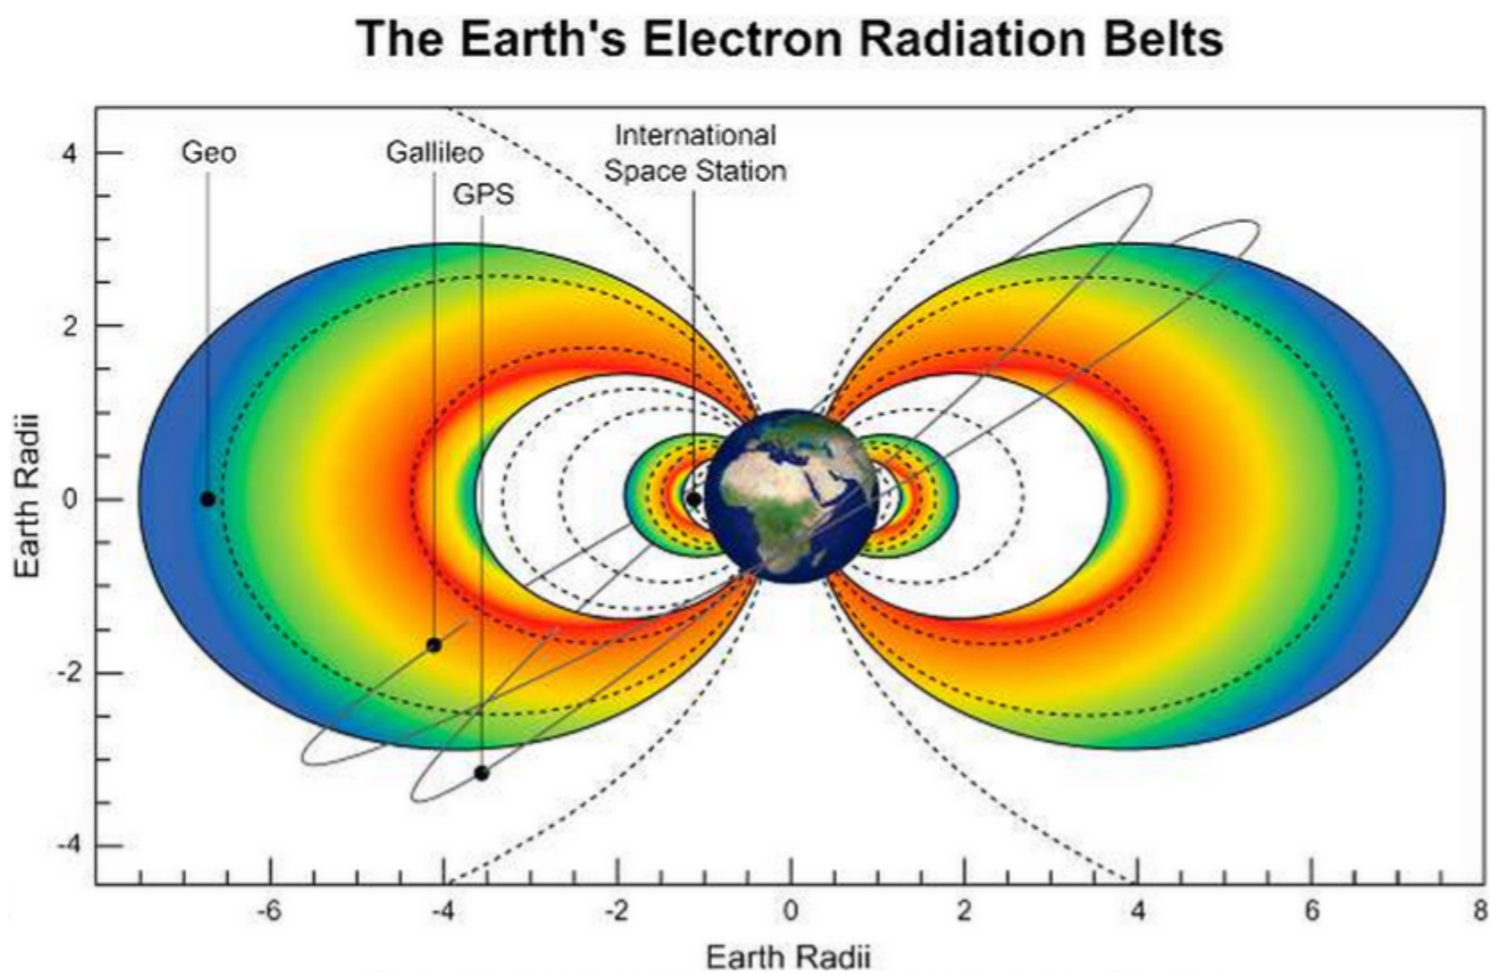
\includegraphics[width=\textwidth]{1_rad_belt.png}
\caption{The two radiation belts with a the locations of various satellites and orbits. Figure from \citep{Horne2013}.}
\label{Intro:rad_belts}
\end{figure}

\begin{figure}
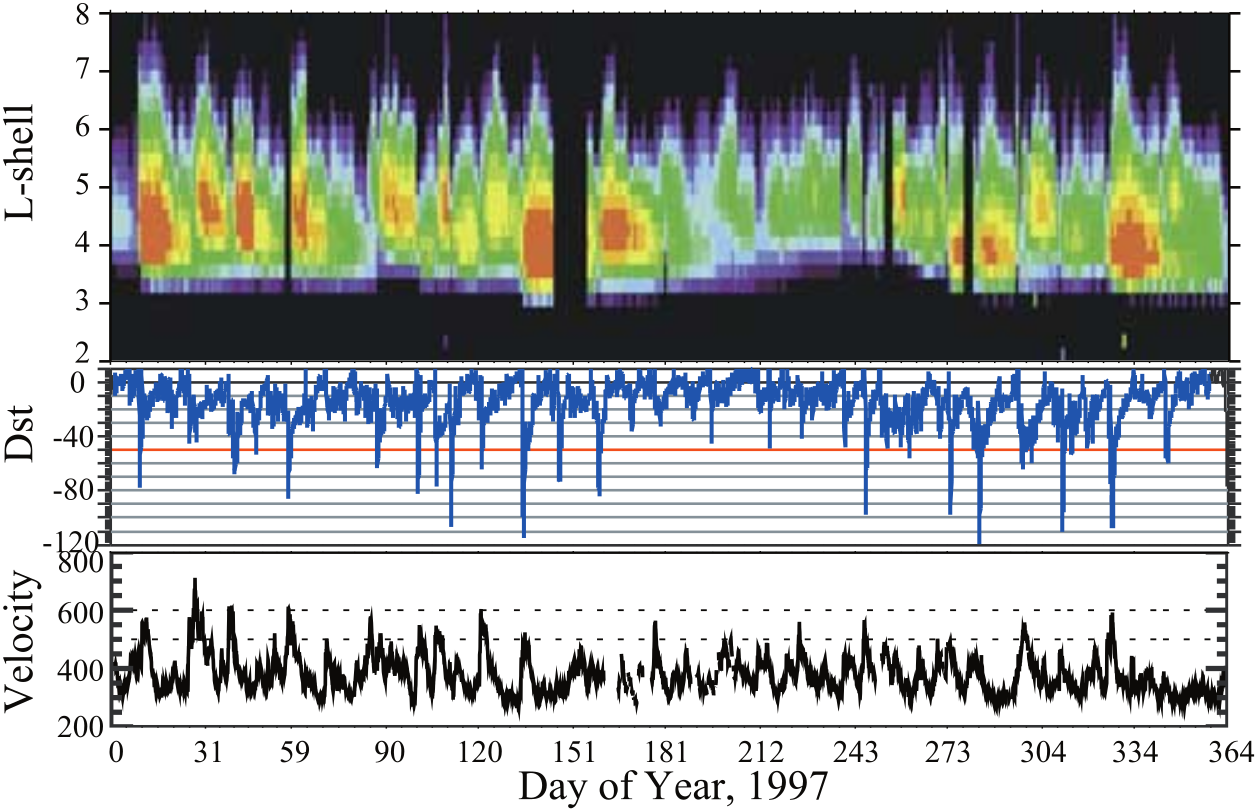
\includegraphics[width=\textwidth]{1_reeves_l_cut.png}
\caption{The dynamics of the outer radiation belt in 1997 from the POLAR satellite. Top panel shows the 1.2-2.4 MeV electron flux as a function of L and 1997 day of year. The middle panel shows the DST index, and bottom panel shows the solar wind velocity. Figure from \citep{Reeves2003}.}
\label{Intro:reeves_l_cut}
\end{figure}

The inner radiation belt is extremely stable on time periods of years, extends to $L \approx 2$, and mainly consists of protons with energies between MeV and GeV and electrons with energies up to $\approx 1$ MeV \citep{Claudepierre2019}. The source of inner radiation belt protons is believed to be due to cosmic-ray albedo neutron decay \citep[e.g.][]{Li2017_CRAND} and inward radial diffusion for electrons \citep[e.g.][]{O'Brien2016_inner}. The gap between the inner and outer radiation belt is called the slot, which is believed to be due to hiss waves inside the plasmasphere (described below) scattering particles into the atmosphere \citep[e.g.][]{Lyons1973, Breneman2015}.

The outer radiation belt is much more dynamic and consists of mainly electrons of energies up to a few MeV. The outer belt's spatial extent is highly variable as shown in Fig. \ref{Intro:reeves_l_cut}, and is typically observed between L of $4$ and $8$. The source of outer radiation belt electrons is widely believed to be injections of plasma from the magnetotail that is then accelerated to high energies.

Due to the highly energetic and dynamic nature of the radiation belts, and their impact on space exploration, the radiation belts have been studied for over half century. Researchers have studied and attempted to predict the dynamics of radiation belt particles, waves, and wave-particle interactions by considering various competing particle acceleration and loss mechanisms \textcolor{red}{which are described next}.

\section{Radiation Belt Particle Sources and Sinks}\label{Intro:sources_sinks}
In the magnetosphere there are a variety of mechanisms that transport, energize, and/or remove particles. As is shown in Fig. \ref{Intro:reeves_l_cut}, the radiation belt particle fluxes vary wildly which correspond to times when either loss or acceleration mechanisms dominate. In this section we will discuss a few mechanisms that contribute to this balance of particle sources of sinks, including adiabatic heating, wave-resonance heating, magnetopause shadowing, and wave-particle scattering.

\subsection{Adiabatic Heating}\label{Intro:adiabatic_heating}
One of the particle heating and transport mechanisms arises from the Earthward convection of particles. As shown in Eq. \ref{j1_conservation}, the conservation of $J_1$ implies that the initial and final $v_\perp$ depends on the change in the magnetic field magnitude. As a particle convents Earthward $B_f > B_i$ and thus $v_\perp$ must also increase. The dipole magnetic field magnitude in micro Tesla $(\mu T)$ can be written as

\begin{equation}
B(L, \theta) = \frac{31.2 \ \mathrm{\mu T}}{L^3}\sqrt{1 + 3 \cos^2 \theta}.
\end{equation} The change in $v^2_{\perp}$ can be found by taking the ratio of $B(L, \theta)$ at two different $L$ shells

\begin{equation}
\frac{v_{\perp \ f}^2}{v_{\perp \ i}^2} = \bigg( \frac{L_i}{L_f} \bigg)^3
\end{equation} thus the increase in $v_\perp \sim (L_i/L_f)^{3/2}$.

As the particle convects Earthward its $v_{||}$ also increases because the distance between the particle's mirror points decrease. If $J_2$ is conserved, the shrinking bounce path implies that $v_{||}$ must increase by 

\begin{equation}
\frac{v_{|| \ f}^2}{v_{|| \ i}^2} = \bigg( \frac{L_i}{L_f} \bigg)^k
\end{equation} where $k$ ranges from $2$ for equatorial pitch angles, $\alpha_{eq} = 0^\circ$, to $2.5$ for $\alpha_{eq} = 90^\circ$ \citep{Baumjohann1997}. Since the rate of adiabatic heating is greater in the perpendicular direction than heating in the parallel direction, an initially isotropic particle distribution will become anisotropic during its convection. These isotropic particles can then become unstable to wave growth and generate waves in order to reach equilibrium.


\subsection{Wave Resonance Heating}\label{Intro:wave_heating}
Another mechanism that heats particles is due to particles resonating with plasma waves. A few of the electromagnetic wave modes responsible for particle acceleration (and scattering) relevant to radiation belt dynamics are hiss, whistler mode chorus (chorus), and electromagnetic ion cyclotron (EMIC) waves. These waves are created by the loss cone instability that is driven by an anisotropy of electrons for chorus waves, and protons for EMIC waves. The level of anisotropy can be quantified by the ratio of the perpendicular to parallel particle temperatures $(T_\perp/T_{||})$. A particle distribution is unstable when $T_\perp/T_{||} > 1$. Since electrons gyrate in a right-handed sense, the chorus waves also tend to be right hand circularly polarized \citep{Tsurutani1997}. The same argument also applies to protons and left hand circularly polarized EMIC waves. 

These circularly polarized waves can resonate with electrons and/or protons when their relative motion results in a static $\vec{E}$. One example of a resonance between a right hand circularly polarized wave and an electron is shown in Fig. \ref{Intro:resonance_diagram}. The electron's $v_{||}$ and the wave's parallel wave vector, $k_{||}$ are in opposite directions such that the wave frequency $\omega$ is Doppler shifted to an integer multiple of the $\Omega_e$ where the electron feels a static electric field and is accelerated or decelerated. Quantitatively, this resonance condition is easier to understand with the following toy model.

\begin{figure}
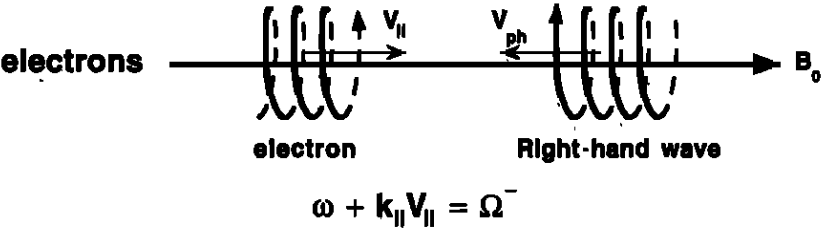
\includegraphics[width=\textwidth]{1_resonance.png}
\caption{The trajectories of an electron and a right-hand circularly polarized wave during a cyclotron resonance. The electron's $v_{||}$ and the wave's $k_{||}$ are in opposite directions such that the wave's frequency is Doppler shifted to a integer multiple of the electron cyclotron frequency. Figure from \citep{Tsurutani1997}.}
\label{Intro:resonance_diagram}
\end{figure}

Assume a uniform magnetic field $\vec{B} = B_0 \hat{z}$ with a parallel propagating ($k = k\hat{z}$), right-hand circularly polarized wave. The wave's electric field as a function of position and time can be written as

\begin{equation}
\vec{E} = E_0 (\cos{(\omega t - kz)}\hat{x} + \sin{(\omega t - kz)}\hat{y}).
\end{equation} The angular component of $\vec{E}$ that will effect the particle's $v_\perp$ is 
\begin{equation}
E_\theta = \vec{E} \cdot \hat{\theta} = E_0 \cos{(\omega t - kz + \theta)}.
\end{equation} Now assume that the electron is traveling in the $-\hat{z}$ direction with a velocity $\vec{v} = -v_0 \hat{z}$ so its time dependent position along $\hat{z}$ is

\begin{equation}
z(t) = -v_0 t
\end{equation} and gyrophase is

\begin{equation}
\theta(t) = -\Omega t + \theta(0)
\end{equation} where the first negative sign comes from the electron's negative charge. Now we put this all together and find the force that the electron will experience

\begin{equation}
m \frac{dv_\theta}{dt} = qE_\theta = qE_0 \sin{((\omega + kv_0 - \Omega)t + \theta(0))}.
\end{equation} This is a relatively complex expression, but when the time dependent component is 0, i.e. 

\begin{equation} \label{Intro:resonance}
\omega + kv_0 - \Omega = 0,
\end{equation} the electron will feel a static electric field and be accelerated or decelerated depending on $\theta_0$, the phase between the wave and the electron. The expression in Eq. \ref{Intro:resonance} is commonly referred to as the resonance condition and is more generally written as 

\begin{equation} \label{Intro:resonance_general}
\omega - k_{||} v_{||} = \frac{n \Omega_e}{\gamma}
\end{equation} where $n$ is the resonance order, and $\gamma$ is the relativistic correction \citep[e.g.][]{Millan2007}. In the case of the cyclotron resonance, $\omega \approx \Omega_e$ thus $J_1$ is violated. Since $J_1$ is violated, $J_2$ and $J_3$ are also violated since the conditions required to violate $J_2$ and $J_3$ are less stringent than $J_1$. It is important to remember that a particle will experience the effects of many waves along its drift orbit. The typical MLT extent of a handful of waves that are capable of resonating with radiation belt electrons are shown in Fig. \ref{Intro:waves}.

\begin{figure}
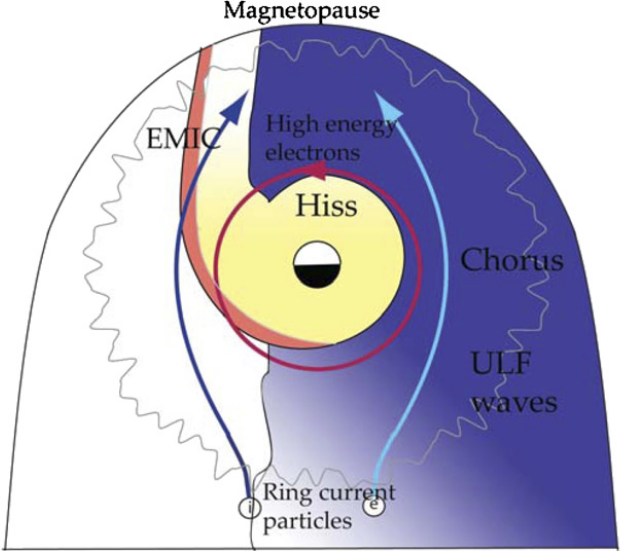
\includegraphics[width=\textwidth]{1_wave_populations.png}
\caption{Various wave modes in the magnetosphere. Ultra low frequency waves occur throught the magnetosphere. Chorus waves are typically observed in the 0-12 midnight-dawn region. EMIC waves are typically observed in the dusk MLT sector. Hiss waves are observed inside the plasmasphere. Figure from \citet{Millan2007}.}
\label{Intro:waves}
\end{figure}

\subsection{Particle Losses}\label{Intro:losses}
Now that we have seen two general mechanisms with which particles are accelerated in the magnetosphere, we will now consider a few specific mechanisms that remove particles from the magnetosphere into the atmosphere or the solar wind. One mechanism that transports magnetosperic particles into the solar wind is magnetopause shadowing \citep[e.g.][]{Ukhorskiy2006}. Magnetopause shadowing occurs when the ring current is strengthened and Earth's magnetic field strength is increased outside of the ring current. If the ring current increases slowly enough (such that $J_3$ is conserved), a particle drift shell will move outward to conserve $J_3$. If the particle's drift shell expands past the magnetopause, the particle will be lost to the solar wind.

\textcolor{red}{Make sure I understand ULF waves and radial diffusion right}
Another particle loss (and acceleration) mechanism is driven by ultra low frequency (ULF) waves and is called radial diffusion. Radial diffusion is the transport of particles from high to low phase space density, $f$. If the transport is radially inward, particles will appear to be accelerated. On the other hand, radially outward radial diffusion can transport particles through the magnetopause where they will be lost to the solar wind. \citet{Reeves2013} investigated the driver of particle acceleration during the October 2012 storm and observationally found that inward radial diffusion was not dominant, rather local acceleration via wave-resonance heating appeared to be the dominant acceleration mechanism.

The loss mechanism central to this dissertation is pitch angle and energy scattering of electrons by waves. Some of the waves that scatter electrons in energy and pitch angle in the inner magnetosphere are: plasmaspheric hiss \citep[e.g.][]{O'Brien2014, Breneman2015}, EMIC waves \citep[e.g.][]{Hendry2017, Capannolo2019energetic}, and chorus waves \citep[e.g.][]{Breneman2017, Kasahara2018, Ozaki2019}. These wave-particle interactions occur when the resonance condition in Eq. \ref{Intro:resonance_general} is satisfied and the particle's energy and $\alpha$ is modified by the wave. More details regarding the theory of pitch angle and energy diffusion is given in Chapter \ref{CH:mageis_microburst}. If the wave changes $\alpha$ towards $0$ and $\alpha < \alpha_{L}$, then the particle's mirror point dips below $100$ km altitude where the particle can be lost from the magnetosphere. One manifestation of pitch angle scattering of particles into the loss cone are microbursts: a sub-second durtaion impulse of electrons.

\section{Microbursts}\label{Intro:microbursts}
Microbursts were first with high altitude balloons which measured bremsstrahlung X-rays emitted by microburst electrons impacting the atmosphere by \citet{Anderson1964}. In the following years, numerous balloon flights expanded our knowledge of non-relativistic (< 500 keV) microbursts (relativistic microbursts have not yet been observed by high altitude balloons) by quantifying the microburst spatial extent, temporal width, occurrence frequency, extent in L and MLT, and their source. The microburst source was first believed to be either a local plasma instability or a propagating disturbance in the magnetosphere \citep{Trefall1966, Brown1965_2, Barcus1966, Parks1967}. Soon after, both non-relativistic and relativistic microbursts electrons were directly observed in LEO with spacecraft including the Solar Anomalous and Magnetospheric Particle Explorer (SAMPEX) \citep[e.g.][]{Blake1996, Blum2015, Lorentzen2001a, Lorentzen2001b, Nakamura1995, Nakamura2000, O'Brien2003, O'Brien2004, Greeley2019, Douma2017, Douma2019},  Montana State University's (MSU) Focused Investigation of Relativistic Electron Bursts: Intensity, Range, and Dynamics II (FIREBIRD-II) \citep{Spence2012, Klumpar2015, Crew2016, Anderson2017, Breneman2017}, and Science Technologies Satellite (STSAT-I) \citep[e.g.][]{Lee2005, Lee2012}. An example microburst time series is shown in Fig. \ref{Intro:microbursts} and was observed by the FIREBIRD-II CubeSats. The prominent features of the example microbursts in Fig. \ref{Intro:microbursts} are their sub-second duration, half order of magnitude increase in count rate above the falling background, and their 200-800 keV energy extent.

\begin{figure}
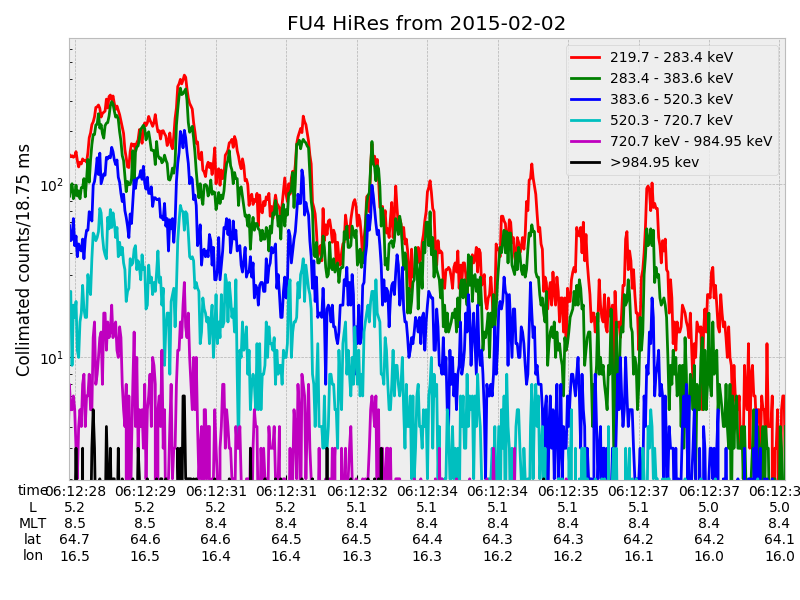
\includegraphics[width=\textwidth]{1_microbursts.png}
\caption{An example train of microbursts observed by FIREBIRD-II unit 4 on February 2nd, 2015. The colored curves show the differential energy channel count rates in five channels from $\approx 200$ keV to 1 MeV and a sixth integral energy channel with a 1 MeV threshold. The x-axis labels show auxiliary information such as time of observation and the spacecraft position in L, MLT, latitude and longitude coordinates.}
\label{Intro:microbursts}
\end{figure}

\begin{figure}
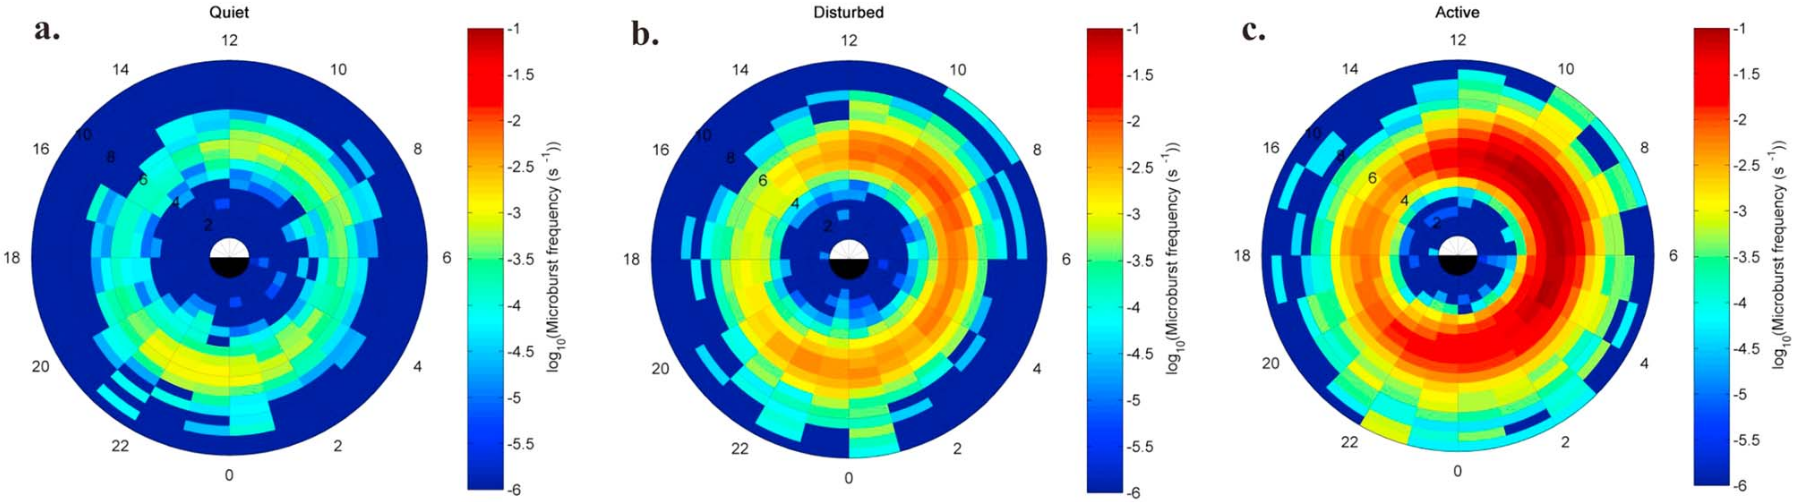
\includegraphics[width=\textwidth]{1_microburst_distribution_douma.png}
\caption{Distribution of $> 1$ MeV microburst occurrence rates as a function of L and MLT. The three panels show the microburst occurrence rate dependence on geomagnetic activity, parameterized by the auroral electrojet (AE) index for (a) $\mathrm{AE} < 100$ nT, (b) $100 < \mathrm{AE} < 300$ nT and (c) $\mathrm{AE} > 300$ nT. Figure from \citet{Douma2017}.}
\label{Intro:microburst_distribution}
\end{figure}

Microbursts are observed on magnetic field footprints that are connected to the outer radiation belt (approximately $4 < L < 8$). They are predominately observed in the 0-12 MLT sector with an elevated occurrence frequency during magnetospherically disturbed times as shown in Fig. \ref{Intro:microburst_distribution} \citep[e.g.][]{Douma2017}. \citet{O'Brien2003} used SAMPEX relativistic electron data and found that microbursts predominately occur during the main phase of storms, with a heightened occurrence rate during the recovery phase. Microburst occurrence rates are also higher during high solar wind velocity events e.g. from co-rotating interaction regions \citep{O'Brien2003, Greeley2019}.

The estimated impact of microbursts on the atmosphere and the radiation belts is significant. Relativistic microburst electrons impacting the atmosphere are ionized at $<100$ km altitudes, with higher energy electrons penetrating closer to the surface. The resulting chemical reaction of microburst electrons impacting the atmosphere produces odd hydrogen $\mathrm{HO_x}$ and odd nitrogen $\mathrm{NO_x}$ molecules, which are partially responsible for destroying ozone ($\mathrm{O_3}$). \citet{Seppala2018} modeled a six hour relativistic microburst storm and found that the mesospheric ozone was reduced by $7-12 \%$ in the summer months and $12-20 \%$ in the winter months, so microbursts may have a non-negligible contribution to the dynamics of atmospheric ozone. Furthermore, microbursts have also been estimated to have a significant impact on the outer radiation belt electron population. Radiation belt electron loss due to microbursts has been estimated to be on the on the order of a day \citep{Lorentzen2001b, O'Brien2004, Thorne2005, Breneman2017, Douma2019}. 

The wave-particle interactions responsible for generating microbursts are also believed to accelerate electrons in the radiation belts. As mentioned earlier, when an electron is in resonance with a wave, energy is exchanged with the wave and the electron is either accelerated or decelerated. The signature of wave-particle acceleration been observed for radiation belt electrons \citep[e.g.][]{Meredith2002, Horne2005, Reeves2013}, and \citet{O'Brien2003} presented evidence that enhancements in chorus waves, microbursts, and radiation belt electrons are related. To explain their observations, \citet{O'Brien2003} proposed that microburst precipitation is a side effect of electron acceleration due to chorus waves. 

The widely used theoretical framework to model the wave-particle interactions responsible for accelerating electrons and scattering microbursts is quasi-linear diffusion \citep[e.g.][]{Walker1993, Summers1998, Meredith2002, Horne2005, Thorne2005, Summers2005}. This framework is explained in Chapter \ref{CH:mageis_microburst}, and applied to an observation of a microburst in the heart of the radiation belt. Qualitatively, when a particle is resonant with a wave it can either be transported in pitch angle towards the loss cone and lose energy to the wave, or transported away from the loss cone and gain energy from the wave.

As previously mentioned, the range of observed microburst energies range from a few tens of keV \citep[e.g][]{Datta1997, Parks1967} to greater than 1 MeV \citep[e.g.][]{Blake1996, Greeley2019}. The microburst electron flux ($J$) falls off in energy, and the microburst energy spectra is typically well fit to a decaying exponential 

\begin{equation}
J(E) = J_0 e^{-E/E_0}
\end{equation} where $J_0$ is the flux at 0 keV (unphysical free parameter) and $E_0$ quantifies the efficiency of the scattering mechanism in energy \citep[e.g.][]{Parks1967, Datta1997, Lee2005}. A small $E_0$ suggests that mostly low energy particles are scattered. In contrast a high $E_0$ suggests that the scattering mechanism scatters low and high energy electrons. Reality is a bit more messy and a high $E_0$ may be a signature of a scattering mechanism preferential to high energy electrons, but is hidden by the convolution of the source particles available to be scattered (typically with a falling energy spectrum) and the energy-dependent efficiency of the scattering mechanism.

The short microburst duration observed by a single LEO satellite has an ambiguity when interpreting what is exactly a microburst. The two possible realities are: a microburst is very small and spatially stationary so that the LEO spacecraft passes through it in less than a second. Alternatively, microbursts are spatially large and transient so a microburst will pass by the spacecraft in a fraction of a second. There are a few ways to distinguish between the two possible realities, and each one has a unique set of advantages.

A high altitude balloon provides essentially a stationary view of the precipitating particles under the radiation belt footprints. A short-lived, temporal microburst can be unambiguously identified. Spatial structures, on the other hand, are difficult to identify because a balloon is essentially still on drift timescales.

Multi-spacecraft missions are an alternate solution that can determine if a microburst is spatial or temporal. As will be shown in this dissertation, if a microburst is observed simultaneously by two spacecraft then it is temporal and has a size greater than the spacecraft separation. On the contrary, if two spacecraft observe a microburst-like feature at different times but at the same location, then the feature is spatial and may be a curtain \citep{Blake2016}. Both balloon and multi-spacecraft observational methods have a unique set of strengths, and this dissertation takes the multi-spacecraft approach to identify and study microbursts.


\section{Scope of Reserach}\label{Intro:scope}
This dissertation furthers our understanding of the microburst scattering mechanism by presenting observational evidence of microburst scattering directly, and measuring microburst sizes and comparing them to the size of chorus waves. Chapter \ref{CH:mageis_microburst} describes a microburst scattering event observed by NASA's Van Allen Probes. For this event, particle and wave measurements were analyzed and modeled in the theoretical framework of pitch angle and energy diffusion. Then the following two chapters present studies of microburst sizes in comparison to chorus waves. Chapter \ref{CH:bouncing_packet} describes a bouncing packet microburst observation made by the FIREBIRD-II mission where the microburst's lower bound longitudinal and latitudinal sizes were estimated. Then Chapter \ref{CH:ac6_study} expands the case study from Chapter \ref{CH:bouncing_packet} to a statistical study of microburst sizes using The Aerospace Corporation's AeroCube-6 (AC6) CubeSats. In this study, a Monte Carlo and analytic microburst size models were developed to account for the compounding statistical effects of random microburst sizes and locations. Lastly, Chapter \ref{conclusions} will summarize this work and make concluding remarks regarding outstanding questions in microburst physics.